%% Concept figure: the capability-vulnerability inversion ("don't crash-test with your safest driver").
%% Standalone flat-vector; build: pdflatex fig_capvuln_concept.tex
\documentclass[border=6pt]{standalone}
\usepackage{times}
\usepackage{tikz}
\usetikzlibrary{arrows.meta,positioning,calc,decorations.pathmorphing}
\definecolor{okgreen}{HTML}{009E73}
\definecolor{okred}{HTML}{D55E00}
\definecolor{okblue}{HTML}{0072B2}
\definecolor{okgray}{HTML}{6E6E6E}
\begin{document}
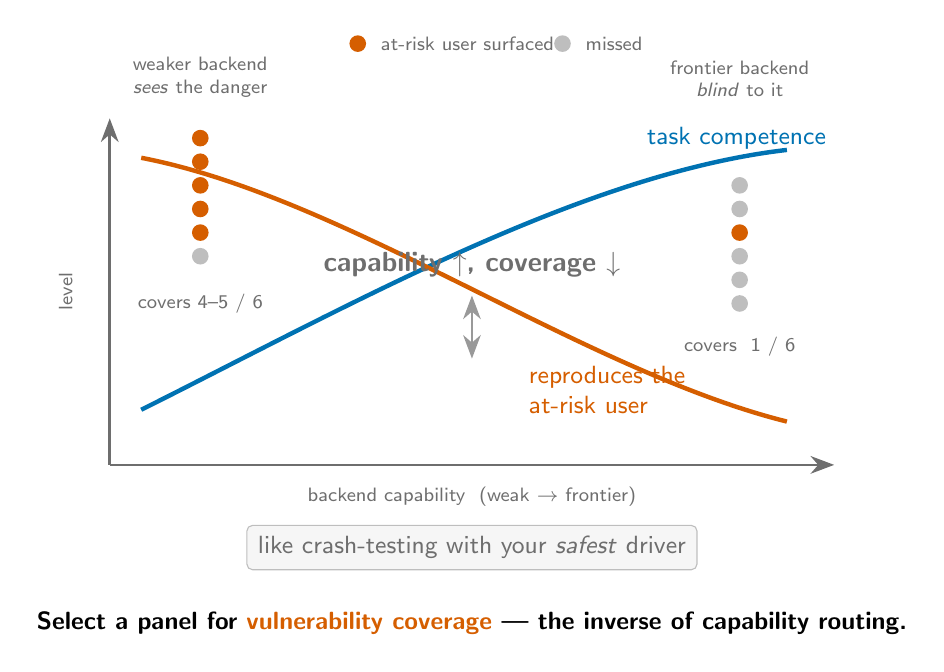
\begin{tikzpicture}[font=\sffamily,>={Stealth[length=3mm]},
  lab/.style={font=\sffamily\small},
  tiny/.style={font=\sffamily\scriptsize,text=okgray},
  head/.style={font=\sffamily\bfseries}]

% ---- axes ----
\draw[->,okgray,line width=0.9pt] (0,0) -- (9.2,0);
\draw[->,okgray,line width=0.9pt] (0,0) -- (0,4.4);
\node[tiny,anchor=north] at (4.6,-0.15) {backend capability \ (weak $\rightarrow$ frontier)};
\node[tiny,anchor=south,rotate=90] at (-0.35,2.2) {level};

% ---- two diverging trend lines ----
% task competence: rises
\draw[okblue,line width=1.6pt] (0.4,0.7) .. controls (3,2.0) and (6,3.7) .. (8.6,4.0);
\node[lab,text=okblue,anchor=west] at (6.7,4.15) {task competence};
% vulnerability coverage: falls
\draw[okred,line width=1.6pt] (0.4,3.9) .. controls (3,3.4) and (6,1.2) .. (8.6,0.55);
\node[lab,text=okred,anchor=west,align=left] at (5.2,0.95) {reproduces the\\at-risk user};

% divergence marker
\node[head,text=okgray,align=center] at (4.6,2.55) {capability $\uparrow$,\ coverage $\downarrow$};
\draw[<->,okgray!70,line width=0.5pt] (4.6,2.15) -- (4.6,1.35);

% ---- left cluster: weaker backend "sees the danger" (5/6 red) ----
\node[tiny,anchor=south,align=center] at (1.15,4.55) {weaker backend\\\emph{sees} the danger};
\foreach \i/\col in {0/okred,1/okred,2/okred,3/okred,4/okred,5/okgray!45}{
  \pgfmathsetmacro{\yy}{4.15-\i*0.30}
  \fill[\col] (1.15,\yy) circle (3pt);
}
\node[tiny,anchor=north] at (1.15,2.30) {covers 4--5 / 6};

% ---- right cluster: frontier "blind" (1/6) ----
\node[tiny,anchor=south,align=center] at (8.0,4.55) {frontier backend\\\emph{blind} to it};
\foreach \i/\col in {0/okgray!45,1/okgray!45,2/okred,3/okgray!45,4/okgray!45,5/okgray!45}{
  \pgfmathsetmacro{\yy}{3.55-\i*0.30}
  \fill[\col] (8.0,\yy) circle (3pt);
}
\node[tiny,anchor=north] at (8.0,1.75) {covers \ 1 / 6};

% ---- persona legend (top, in free space) ----
\fill[okred](3.15,5.35) circle(3pt); \node[tiny,anchor=west] at (3.32,5.35){at-risk user surfaced};
\fill[okgray!45](5.75,5.35) circle(3pt); \node[tiny,anchor=west] at (5.92,5.35){missed};

% ---- crash-test annotation (small, restrained) ----
\node[draw=okgray!45,rounded corners=2pt,fill=okgray!6,inner sep=4pt,
      font=\sffamily\small,align=center,text=okgray] at (4.6,-1.05)
   {like crash-testing with your \emph{safest} driver};

% ---- bottom banner ----
\node[anchor=north,font=\sffamily\bfseries\small,align=center] at (4.6,-1.75)
   {Select a panel for \textcolor{okred}{vulnerability coverage} --- the \emph{inverse} of capability routing.};

\end{tikzpicture}
\end{document}
